\section{Ruta 3: Universidad de Ljubljana}
Los paquetes hacen varios saltos en Buenos Aires (aunque algunos no responden podemos suponer que son en Buenos Aires), luego de lo cual hay un salto de Buenos Aires a Viena. Esto es anormal, ya que el unico cable submarino que conecta Argentina y Europa llega a España. Esto puede deberse a algún tipo de conexión directa entre Viena y dicho cable. Luego hay algunos saltos mas en Europa hasta llegar a destino. Hay un solo salto intercontinental en el mapa, que es el salto Buenos Aires-Viena, este salto es detectado correctamente, pero al igual que en experimentos anteriores hay muchos falsos positivos.


www.uni-lj.si

\begin{tabular}{l | l | l | l | l}
Hop & RTT & IP & Ubicación & Salto Intercontinental\\
1 & 0.0457 & \texttt{192.168.0.1} & Buenos Aires, Argentina & false\\
2 & null & null & null & null\\
3 & null & null & null & null\\
4 & null & null & null & null\\
5 & null & null & null & null\\
6 & 0.1651 & \texttt{200.89.161.81} & Buenos Aires, Argentina & true\\
7 & 0.3778 & \texttt{200.89.165.86} & Buenos Aires, Argentina & true\\
8 & 0.2096 & \texttt{185.70.203.22} & Buenos Aires, Argentina & true\\
9 & 0.3915 & \texttt{195.22.215.168} & Viena, Austria & true\\
10 & 0.4367 & \texttt{195.22.215.199} & Viena, Austria & false\\
11 & 0.5828 & \texttt{77.94.128.25} & Ljubljana, Eslovenia & true\\
12 & 0.3733 & \texttt{77.94.139.210} & Ljubljana, Eslovenia & true\\
13 & 0.4521 & \texttt{91.216.54.245} & Nova Gorica, Eslovenia & true\\
14 & 0.3534 & \texttt{91.223.115.153} & Nova Gorica, Eslovenia & true\\
\end{tabular}

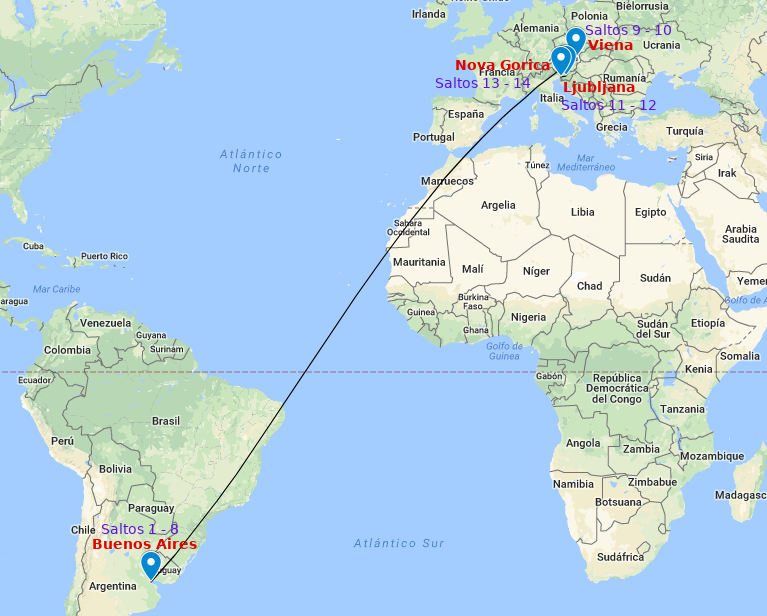
\includegraphics[width=\textwidth]{ljubljana.png}